\begin{figure}[H]
    \centering
         \centering
         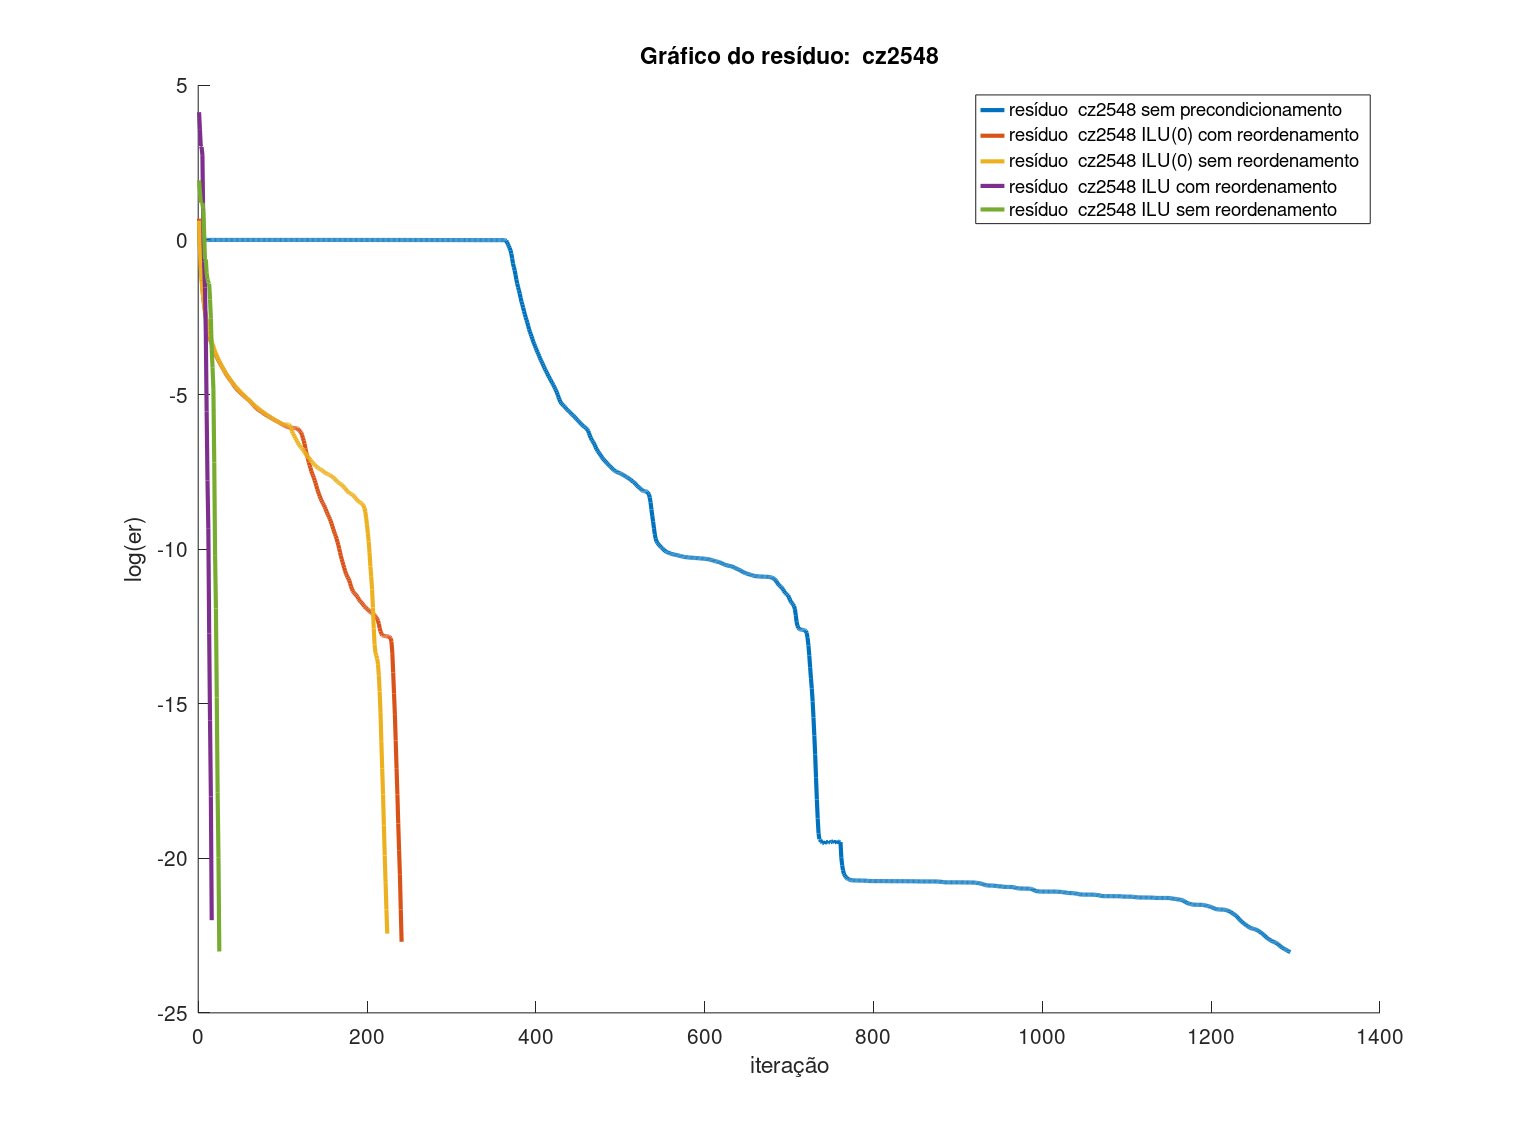
\includegraphics[width=.6\linewidth]{images/cz2548.png}
         \caption{Gráfico do Resíduo da matriz \textit{cz2548}}
         \label{fig:cz-res}
\end{figure}

\begin{figure}[H]
    \centering
         \centering
         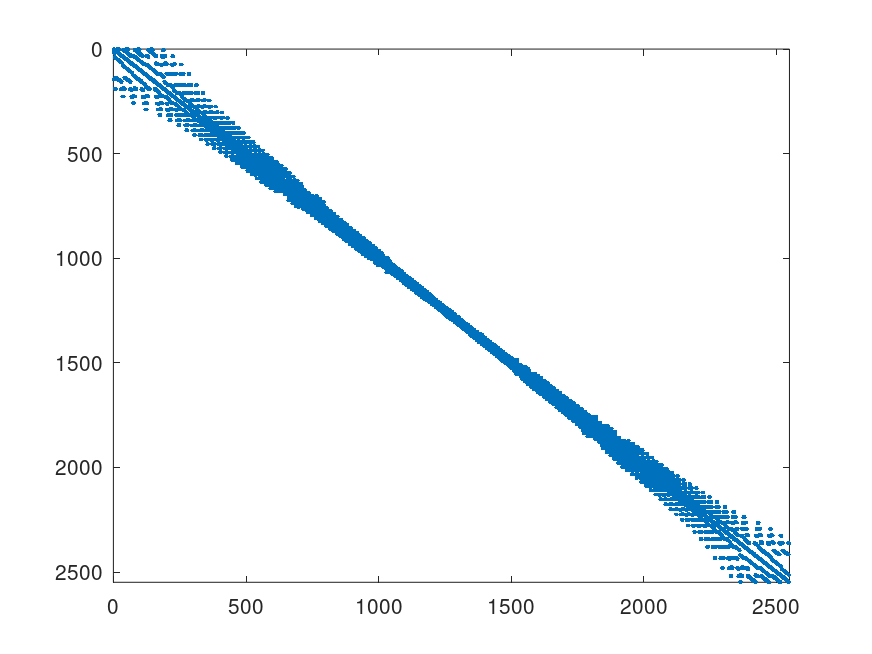
\includegraphics[width=.5\linewidth]{images/cz2548_spyA.png}
         \caption{Spy de da matriz \textit{cz2548}}
         \label{fig:cz-spy-a}
\end{figure}

\begin{figure}[H]
    \centering
    \begin{subfigure}[t]{0.4\linewidth}
         \centering
         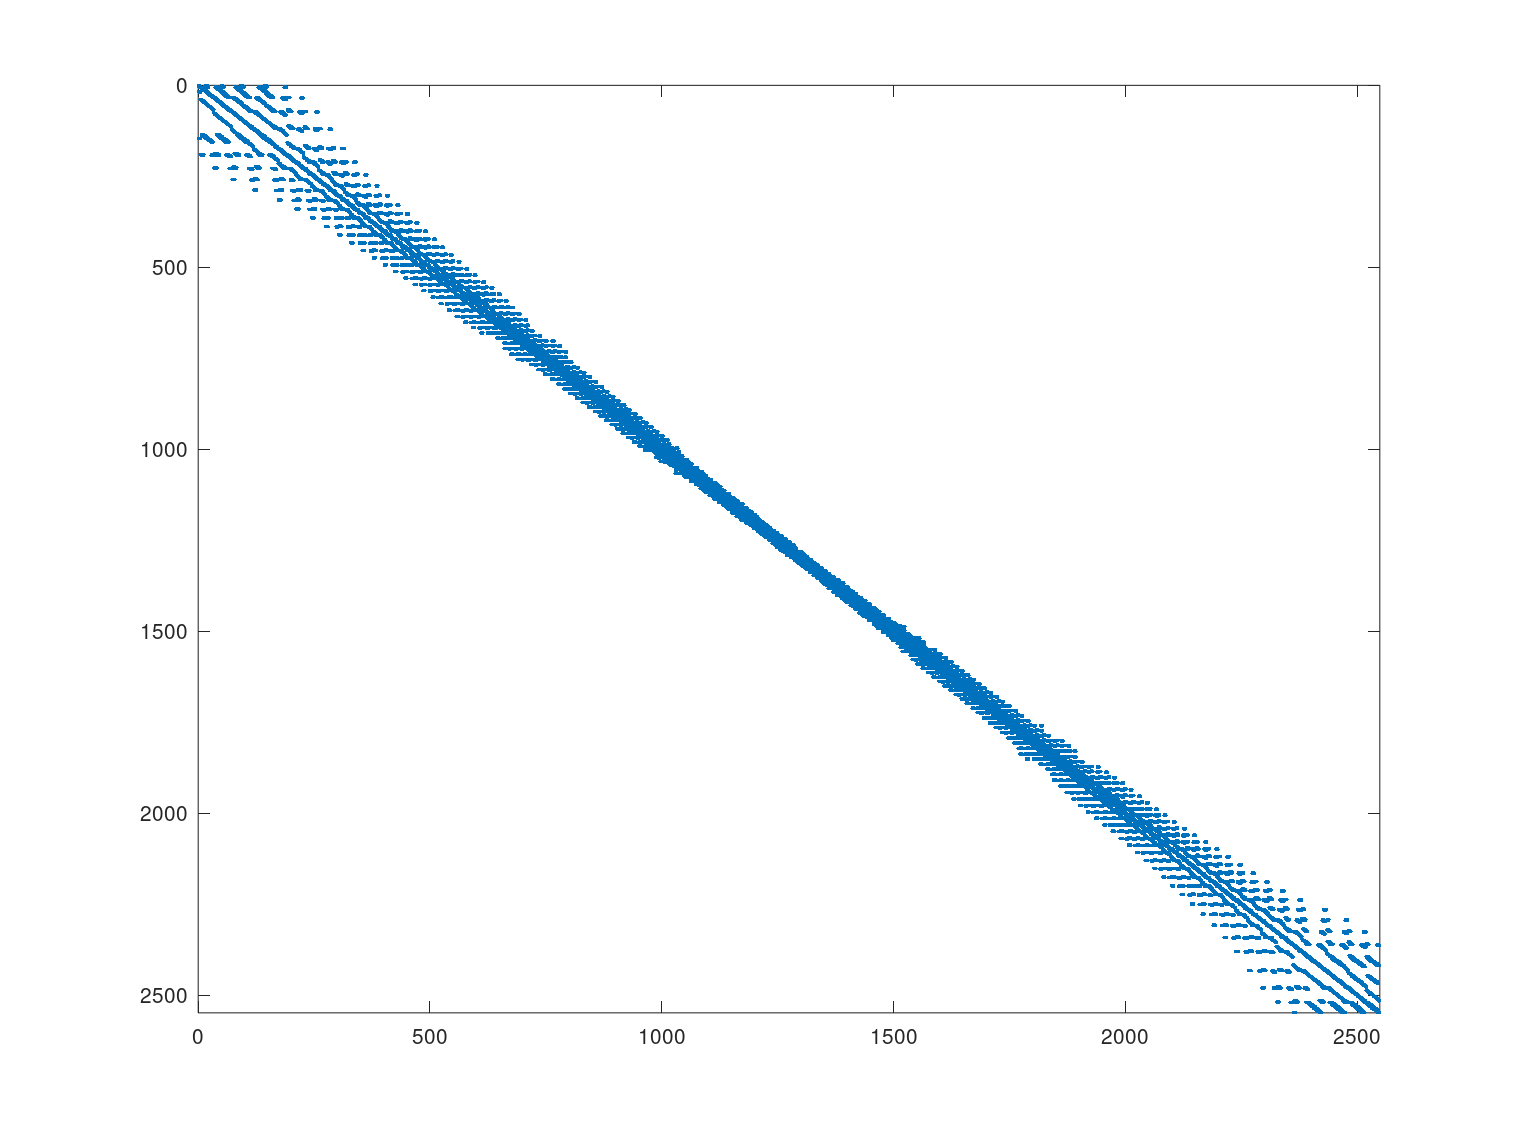
\includegraphics[width=\textwidth]{images/cz2548_spyM_ILU(0)_sem.png}
         \caption{Spy após ILU(0) sem reordenamento}
         \label{fig:cz-ILU0-sem}
    \end{subfigure}
    \quad
    \begin{subfigure}[t]{0.4\linewidth}
         \centering
         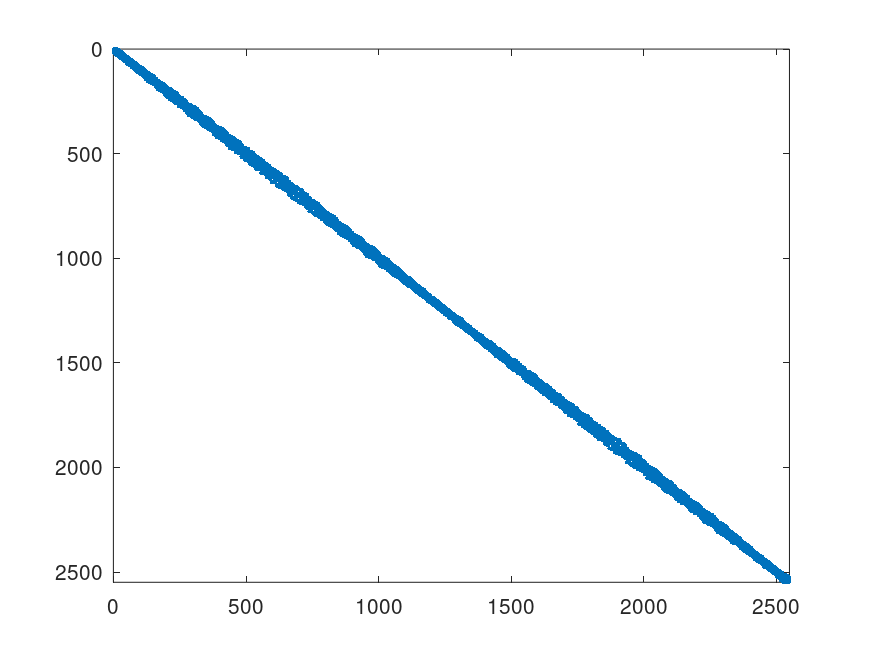
\includegraphics[width=\textwidth]{images/cz2548_spyM_ILU(0)_com.png}
         \caption{Spy após ILU(0) com reordenamento}
         \label{fig:cz-ILU0-com}
    \end{subfigure}
    \par\bigskip
    \begin{subfigure}[t]{0.4\linewidth}
         \centering
         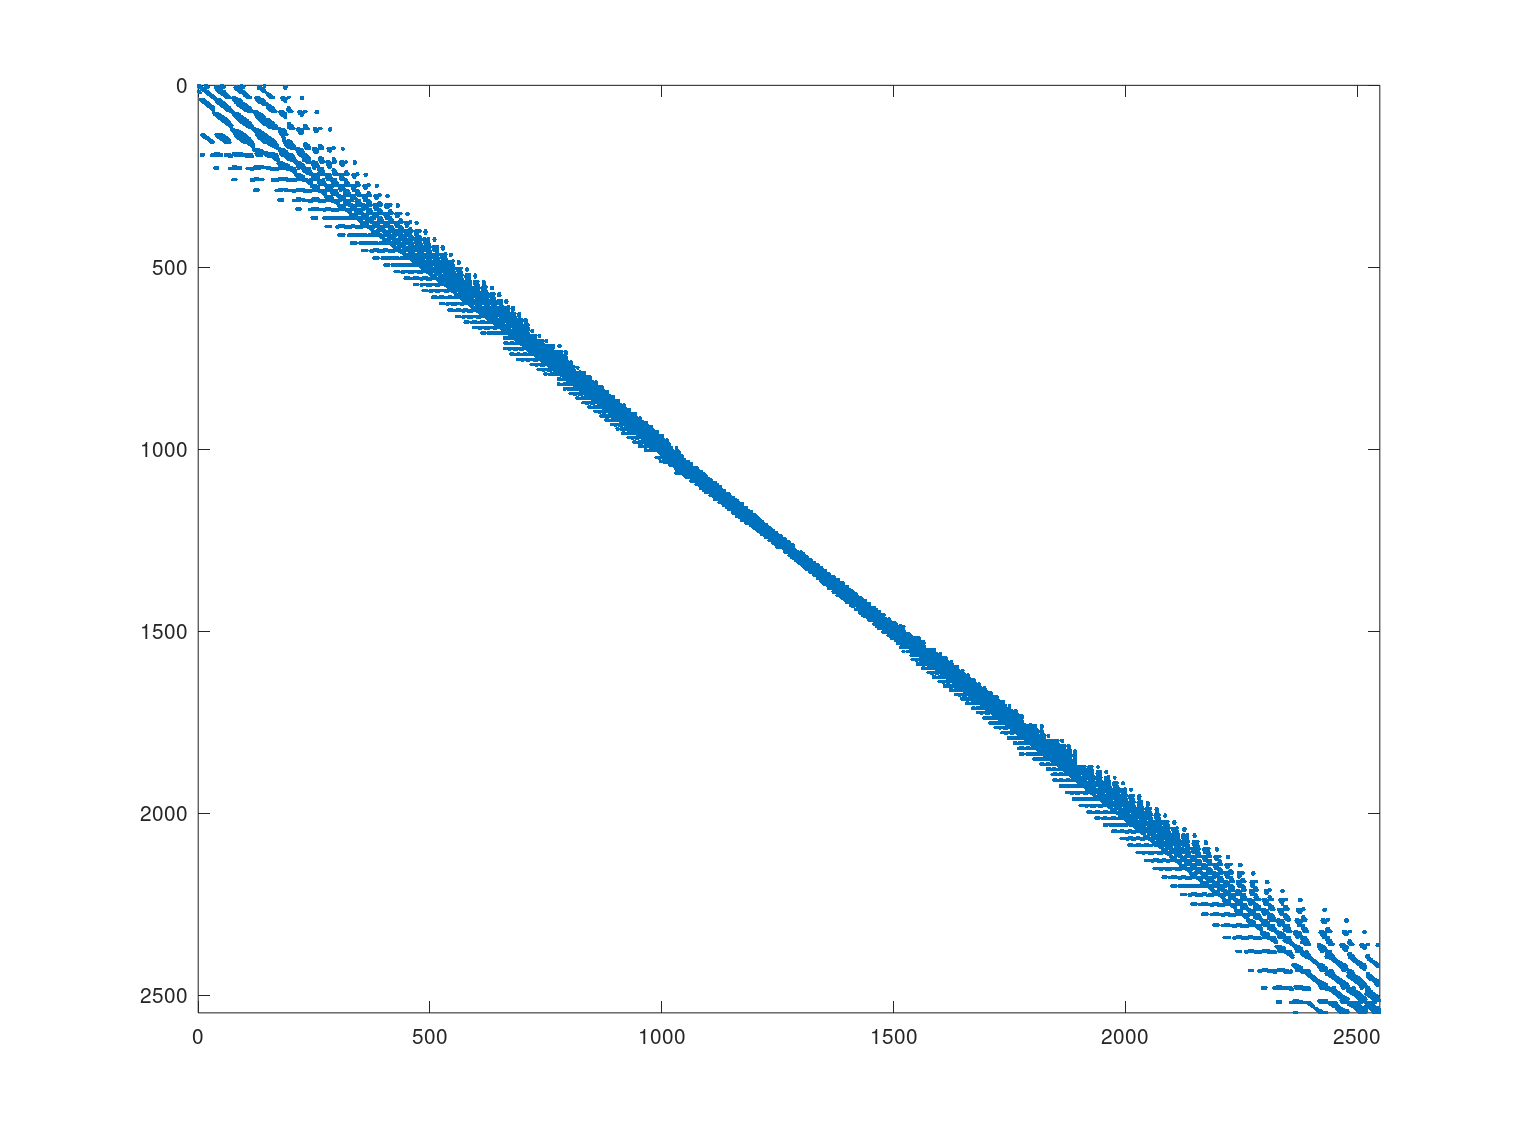
\includegraphics[width=\textwidth]{images/cz2548_spyM_ILU_sem.png}
         \caption{Spy após ILU sem reordenamento}
         \label{fig:cz-ILU-s}
    \end{subfigure}
    \quad
    \begin{subfigure}[t]{0.4\linewidth}
         \centering
         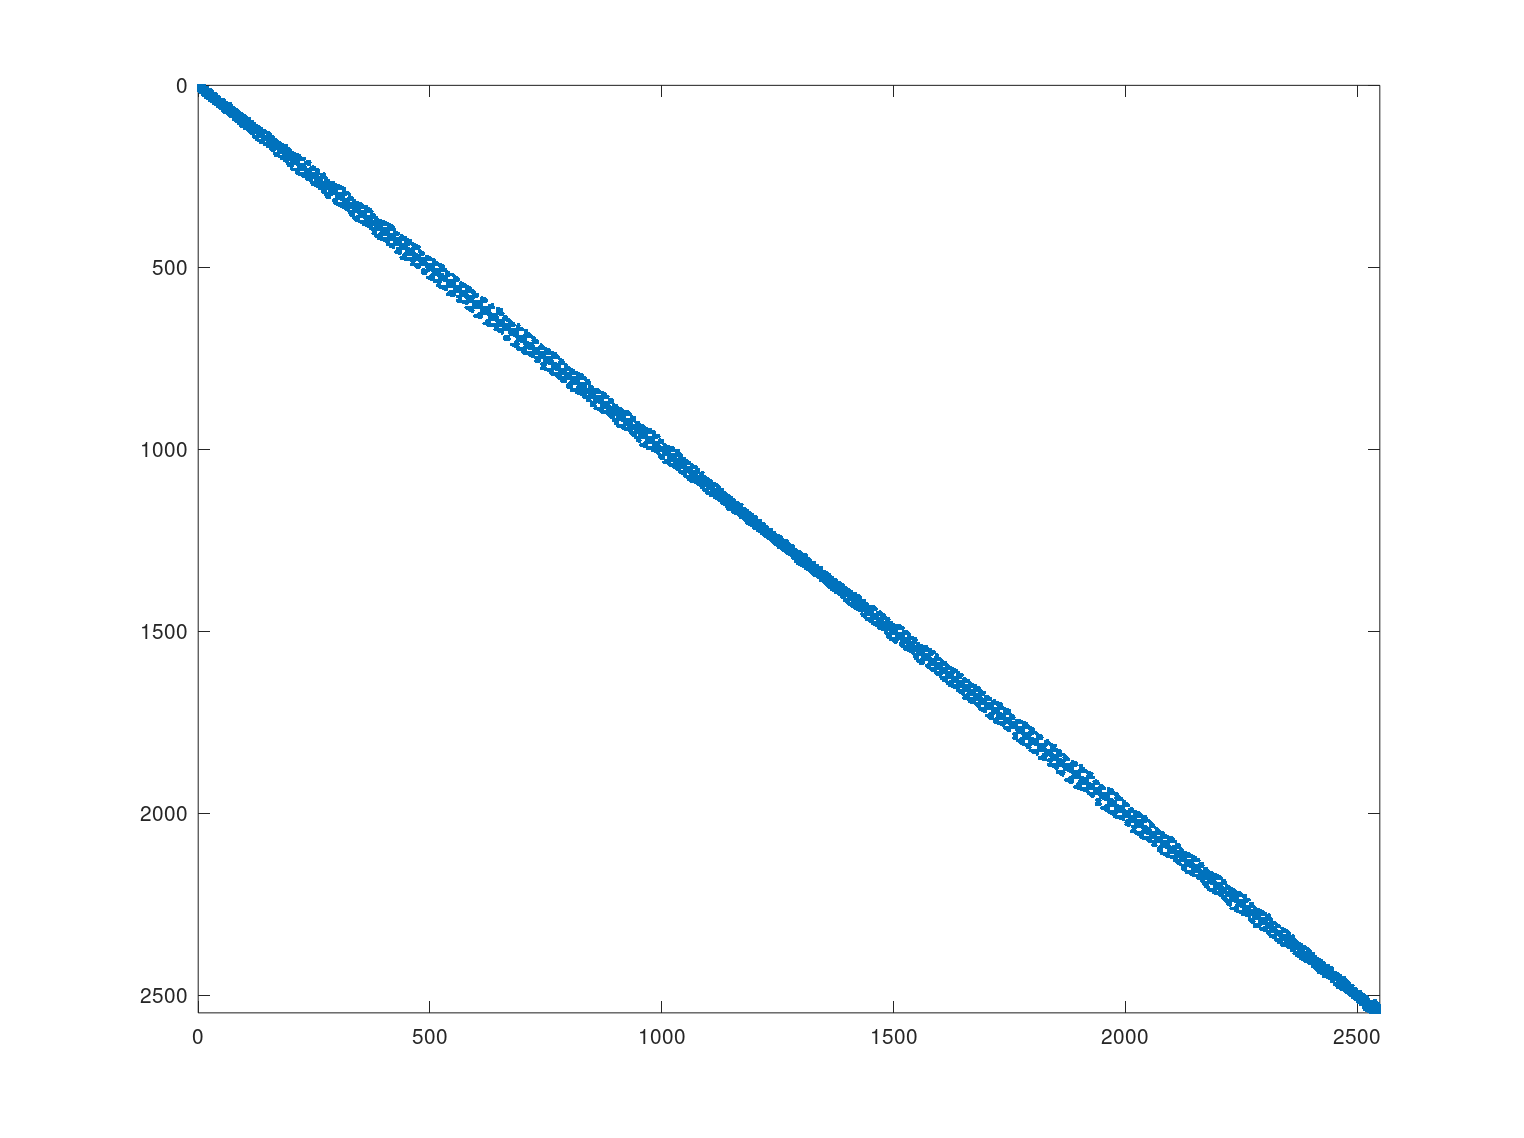
\includegraphics[width=\textwidth]{images/cz2548_spyM_ILU_com.png}
         \caption{Spy após ILU com reordenamento}
         \label{fig:cz-ILU-c}
    \end{subfigure}
    \caption{Gráficos do preenchimento de \textit{cz2548}.}
    \label{fig:cz}
\end{figure}